%=============================================================
\chapter{Trajectory Generation and Planning}
\label{chap:trajectory}
%=============================================================

\section{Overview}

The complete trajectory-tracking stack of the UR5 model can be decomposed into three levels:
\begin{enumerate}
  \item \textbf{Offline trajectory generation}: We implemented a Python script that generates the following files and exports them to CSV
  \begin{itemize}
    \item A smooth Workspace reference trajectory (6D) for the end-effector, defined by a sequence of waypoints and interpolated using \texttt{PCHIP} cubic splines.
    \item A load condition signal that indicates whether the end-effector is carrying a load or not, based on the inter-waypoint segments.
  \end{itemize}
  \item \textbf{Online reference erogation and Workspace-to-Joint mapping}: the CSV is read at each simulation step and the desired end-effector pose is converted to a homogeneous transformation matrix and then mapped to joint angles by the closed-form IK solver.
  \item \textbf{Joint reference conditioning}: the raw IK output is phase-unwrapped to remove $2\pi$ discontinuities, and the resulting continuous joint references are fed to the six PID+G controllers.
\end{enumerate}

The UR5 joints angle is provided by an Integrator block, which does not enforce any bounds on the joint angles. This means that the joint angles can grow indefinitely in either direction, and the controller must be designed to handle this unboundedness. The phase unwrapping step is crucial to ensure that the joint references remain continuous and do not exhibit jumps of $2\pi$ when crossing the $\pm\pi$ boundary.

Figure \ref{fig:traj_chain} illustrates the signal flow from the offline planner through to the low-level controllers.

\begin{figure}[H]
  \centering
  \begin{tikzpicture}[
    >=Stealth,
    every node/.style={font=\small},
    block/.style={draw, rectangle, rounded corners, minimum width=2.6cm,
                  minimum height=0.8cm, align=center, fill=blue!10},
    arrow/.style={->, thick}
  ]
    % Top row (left to right)
    \node[block] (csv)  at (0.0,  0) {CSV File \\ (Python)};
    \node[block] (dff)  at (3.5,  0) {DataFromFile \\ \texttt{EE\_Traj.}};
    \node[block] (plan) at (7.0,  0) {Planner \\ (pose $\to T_{\mathrm{des}}$)};
    \node[block] (ik)   at (10.5, 0) {IK Block \\ (closed-form)};
    % Bottom row (right to left)
    \node[block] (uw)   at (10.5,-2) {Unwrap \\ (phase cont.)};
    \node[block] (pd)   at (7.0, -2) {PID+G \\ Controllers};
    \node[block] (hd)   at (3.5, -2) {Harmonic Drive};
    \node[block] (rb)   at (0.0, -2) {Robot Joint};

    % Forward path
    \draw[arrow] (csv)  -- (dff);
    \draw[arrow] (dff)  -- (plan);
    \draw[arrow] (plan) -- (ik);
    \draw[arrow] (ik)   -- (uw);
    \draw[arrow] (uw)   -- (pd);
    \draw[arrow] (pd)   -- (hd);
    \draw[arrow] (hd)   -- (rb);
    % Feedback
    \draw[arrow] (rb.south) -- ++(0,-0.5)
        -| node[near start, below]{\small $q_i,\dot{q}_i$} (pd.south);
  \end{tikzpicture}
  \caption{Signal chain from offline trajectory generation to motor torque command.}
  \label{fig:traj_chain}
\end{figure}

%-------------------------------------------------------------
\section{Offline Trajectory Generation}
%-------------------------------------------------------------
\subsection{Waypoint Specification}

The end-effector trajectory is defined by a set of $N_w = 11$ waypoints in the six-dimensional Cartesian space $[X,\,Y,\,Z,\,\phi,\,\theta,\,\psi]^\top$, where $(X,Y,Z)$ is the position of the tool-center point in the world frame and $(\phi,\theta,\psi)$ are the XYZ Cardan angles (yaw, pitch, roll) of the end-effector orientation.

The waypoints are sampled at uniformly spaced times over a time horizon of $T_{\text{end}} = 10$ seconds, so that the $k$-th waypoint is defined at time $t_k$ as:
\begin{equation}
  t_k = k \cdot \frac{T_{\text{end}}}{N_w - 1}, \qquad k = 0, 1, \ldots, N_w - 1.
\end{equation}

The waypoints are listed in \cref{tab:waypoints} and encode a motion sequence in which the robot first moves from its rest posture to a sequence of pick-and-place positions.

\begin{itemize}
    \item \textbf{Pre-grasp}: The first three waypoints ($k=0,1,2$) define a motion from the initial pose to a pre-grasp position above the first load.
    \item \textbf{Pick}: The $k=2$ waypoint encodes the load position and the grasping action (load attached at $t_3$).
    \item \textbf{Post-grasp}: The $k=3$ waypoint define the post-grasp position, where the load is lifted up.
    \item \textbf{Transport}: The waypoints from $k=4$ to $k=5$ define a transport motion to the pre-release pose.
    \item \textbf{Pre-release}: The $k=6$ waypoint encodes the pre-release position, where the load is held above the release point.
    \item \textbf{Release}: The $k=7$ waypoint encodes the release position, where the load is detached at $t_7$.
    \item \textbf{Post-release}: The waypoint $k=8$ defines the post-release position, where the end-effector is lifted up after releasing the load.
    \item \textbf{Return to rest}: The last two waypoints ($k=9,10$) define a motion back to the initial rest posture.
\end{itemize}

\begin{table}[H]
  \centering
  \caption{Cartesian waypoints for the end-effector trajectory.}
  \label{tab:waypoints}
  \begin{tabular}{@{}cccccccc@{}}
    \toprule
    $k$ & $X$ [m] & $Y$ [m] & $Z$ [m] & $\phi$ [rad] & $\theta$ [rad] & $\psi$ [rad] & $\text{cond} [\text{bool}]$\\
    \midrule
    0  & $-0.72$ & $-0.11$ & $0.007$  & $\pi/2$ & 0 & 0 & \texttt{False} \\
    1  & $0.00$  & $0.50$  & $0.200$  & $\pi$   & 0 & 0 & \texttt{False} \\
    2  & $0.30$  & $0.00$  & $0.200$  & $\pi$   & 0 & 0 & \texttt{False} \\
    3  & $0.30$  & $0.00$  & $0.050$  & $\pi$   & 0 & 0 & \texttt{True} \\
    4  & $0.30$  & $0.00$  & $0.200$  & $\pi$   & 0 & 0 & \texttt{True}\\
    5  & $0.00$  & $-0.50$ & $0.200$  & $\pi$   & 0 & 0 & \texttt{True}\\
    6  & $-0.30$ & $0.00$  & $0.200$  & $\pi$   & 0 & 0 & \texttt{True}\\
    7  & $-0.30$ & $0.00$  & $0.050$  & $\pi$   & 0 & 0 & \texttt{True}\\
    8  & $-0.30$ & $0.00$  & $0.200$  & $\pi$   & 0 & 0 & \texttt{False}\\
    9  & $0.00$  & $0.30$  & $0.500$  & $\pi$   & 0 & 0 & \texttt{False}\\
    10 & $0.00$  & $0.30$  & $0.500$  & $\pi$   & 0 & 0 & \texttt{False}\\
    \bottomrule
  \end{tabular}
\end{table}

A boolean condition array $\texttt{cond\_sp} \in \{0,1\}^{N_w}$ assigns a load status to each inter-waypoint segment:
segments $[t_3, t_7]$ have $\texttt{Cond} = 1$ (load attached), all others have $\texttt{Cond} = 0$ (free end-effector).
The condition is held constant within each segment.

A graphical representation of the waypoints and the resulting trajectory is provided in \ref{fig:traj_plot}.
\begin{figure}[H]
  \centering
  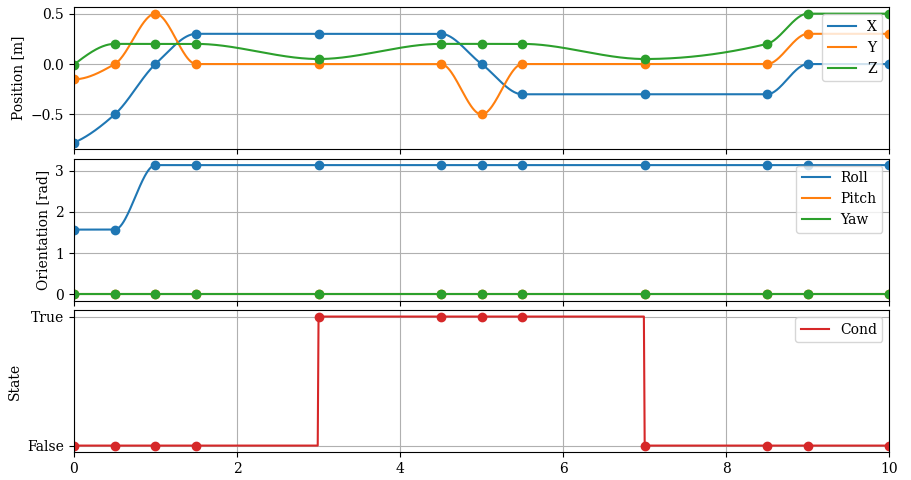
\includegraphics[width=0.9\textwidth]{chapter_trajectory_track/figs/trajectory_reference.png}
  \caption{Visualization of the Workspace Trajectory.}
  \label{fig:traj_plot}
\end{figure}

\subsection{PCHIP Spline Interpolation}

The six Cartesian channels are independently interpolated using a \emph{Piecewise Cubic Hermite Interpolating Polynomial} (PCHIP):
\begin{equation}
  \mathbf{x}(t) = \mathrm{PCHIP}\!\left(\{t_k\},\,\{\mathbf{x}_k\},\,t\right), \qquad \mathbf{x} = [X,\,Y,\,Z,\,\phi,\,\theta,\,\psi]^T.
\end{equation}

PCHIP is preferred over a natural cubic spline because it guarantees \emph{monotonicity preservation}: no spurious oscillations are introduced between waypoints.
This is especially important near the descent phases where large changes in $Z$ occur over a short segment; a standard cubic spline would generate overshoots below the floor level. Moreover, for segments where the pose is held constant, PCHIP reduces to a simple constant interpolation, while a natural cubic spline would still produce small oscillations around the constant value.


The interpolation is performed at a fixed time step $\Delta t = 1$ s, producing a sequence of $N = 100$ Cartesian reference samples.

\subsection{CSV Export}

The trajectory is exported to a comma-separated file with the following columns:
\begin{center}
  \texttt{Time, Cond, X, Y, Z, Roll, Pitch, Yaw}
\end{center}
where \texttt{Cond} is the boolean load flag (as a real $\{0, 1\}$) associated with the time instant according to the segment it belongs to.
The CSV file constitutes the sole interface between the offline Python planner and the 20-sim simulation environment.

%-------------------------------------------------------------
\section{DataFromFile Block and Reference Erogation}
%-------------------------------------------------------------

\subsection{DataFromFile Block}

The \texttt{EE\_Trajectory} block (of type \texttt{DataFromFile}) reads the trajectory CSV at run time samplig at $\Delta t = 1$~s while the simulation integrator typically takes sub-second steps, the DLL performs zero-order hold interpolation between consecutive rows: the reference is held constant until the next data row is reached.
This is consistent with the smooth PCHIP trajectory, which ensures that successive 1-second samples are already close to each other.

The \texttt{Cond} output is cast to a boolean via a \texttt{Cast} block (\texttt{output = (input == 1)}), which converts the real-valued $\{0, 1\}$ CSV column to the boolean type required by the \texttt{X0} and gravity blocks.
A \texttt{Splitter} then fans the boolean out to the \texttt{X0} switching junction, the load gravity source \texttt{g}, and the \texttt{GravityCompensation} block.

\subsection{Pose Assembly}

The six scalar Cartesian channels are re-assembled into a six-element vector \newline $[X,\,Y,\,Z,\,\phi,\,\theta,\,\psi]^T$ by a \texttt{Mux} block, whose output is fed to the \texttt{Planner} block.

The \texttt{Planner} block converts the Euler-angle representation of orientation into a full $4\times 4$ homogeneous transformation matrix $T_{\text{des}}$, using the ZYX convention:
\begin{equation}
  R_{\text{des}} = R_z(\psi)\,R_y(\theta)\,R_x(\phi),
\end{equation}
\begin{equation}
  T_{\text{des}} = \begin{bmatrix} R_{\text{des}} & \mathbf{p}_{\text{des}} \\ \mathbf{0}^T & 1 \end{bmatrix},
\end{equation}
where $\mathbf{p}_{\text{des}} = [X,\,Y,\,Z]^T$ is the desired position.
$T_{\text{des}}$ is then forwarded to the IK block.

%-------------------------------------------------------------
\section{Inverse Kinematics Block}
%-------------------------------------------------------------

\subsection{UR5 Denavit--Hartenberg Parameters}

The closed-form IK solution is based on the standard Denavit--Hartenberg parameterisation of the UR5.
The DH parameters are summarised in \cref{tab:dh}:

\begin{table}[H]
  \centering
  \caption{UR5 Denavit--Hartenberg parameters.}
  \label{tab:dh}
  \begin{tabular}{@{}ccccc@{}}
    \toprule
    Joint $i$ & $\alpha_{i-1}$ [rad] & $a_{i-1}$ [m] & $d_i$ [m] & $\theta_i$ \\
    \midrule
    1 & $0$         & $0$       & $d_1 = 0.089159$  & $\theta_1$ \\
    2 & $\pi/2$     & $0$       & $0$               & $\theta_2$ \\
    3 & $0$         & $a_2 = -0.425$   & $0$      & $\theta_3$ \\
    4 & $0$         & $a_3 = -0.39225$ & $d_4 = 0.10915$ & $\theta_4$ \\
    5 & $\pi/2$     & $0$       & $d_5 = 0.09465$   & $\theta_5$ \\
    6 & $-\pi/2$    & $0$       & $d_6 = 0.0823$    & $\theta_6$ \\
    \bottomrule
  \end{tabular}
\end{table}

\subsection{Analytical Solution}

The IK block implements the closed-form UR5 inverse kinematics.
The desired end-effector transformation $T_{\text{des}} \in \mathrm{SE}(3)$ is decomposed as:
\begin{equation}
  T_{\text{des}} = \begin{bmatrix}
    n_x & o_x & a_x & p_x \\
    n_y & o_y & a_y & p_y \\
    n_z & o_z & a_z & p_z \\
    0   & 0   & 0   & 1
  \end{bmatrix},
\end{equation}
where $\mathbf{n},\,\mathbf{o},\,\mathbf{a}$ are the normal, orientation, and approach unit vectors of the tool frame, and $\mathbf{p}$ is the tool-centre-point position.

The six joint angles are solved in the following order:

\paragraph{Step 1 -- Joint 1 ($\theta_1$).}
The wrist-centre position $\mathbf{p}_{0,5}$ is obtained by offsetting the end-effector position backward along the approach axis by $d_6$:
\begin{equation}
  p_{05x} = p_x - d_6\,a_x, \qquad p_{05y} = p_y - d_6\,a_y.
\end{equation}
The shoulder angle is then:
\begin{align}
  R_s    &= \sqrt{p_{05x}^2 + p_{05y}^2}, \\
  \alpha_1 &= \mathrm{atan2}(p_{05y},\;p_{05x}), \\
  \alpha_2 &= \arccos\!\left(\frac{d_4}{R_s}\right), \\
  \theta_1 &= \alpha_1 + c_s\,\alpha_2 + \frac{\pi}{2},
\end{align}
where $c_s \in \{+1, -1\}$ is the shoulder configuration selector.

\paragraph{Step 2 -- Joint 5 ($\theta_5$).}
The wrist-flip angle follows directly from the projection of the end-effector position onto the $(\sin\theta_1, -\cos\theta_1)$ direction:
\begin{equation}
  \theta_5 = c_w \arccos\!\left(\frac{p_x\sin\theta_1 - p_y\cos\theta_1 - d_4}{d_6}\right),
\end{equation}
where $c_w \in \{+1,-1\}$ is the wrist configuration selector.

\paragraph{Step 3 -- Joint 6 ($\theta_6$).}
From the orientation columns:
\begin{align}
  \theta_6 = \mathrm{atan2}\!\left(
    \frac{-o_x\sin\theta_1 + o_y\cos\theta_1}{\sin\theta_5},\;
    \frac{n_x\sin\theta_1 - n_y\cos\theta_1}{\sin\theta_5}
  \right).
\end{align}

\paragraph{Step 4 -- Sum $\theta_{234} = \theta_2 + \theta_3 + \theta_4$.}
The combined angle of joints 2, 3, and 4 is obtained from the approach vector:
\begin{equation}
  \theta_{234} = \mathrm{atan2}\!\left(-a_z,\;-(a_x\cos\theta_1 + a_y\sin\theta_1)\right).
\end{equation}

\paragraph{Step 5 -- Joints 2 and 3 ($\theta_2$, $\theta_3$).}
An intermediate point $\mathbf{p}_{1,4}$ in the plane of the arm is computed:
\begin{align}
  p_{14x} &= p_{05x}\cos\theta_1 + p_{05y}\sin\theta_1 - d_5\sin\theta_{234}, \\
  p_{14z} &= (p_z - d_6\,a_z) - d_1 + d_5\cos\theta_{234}.
\end{align}
The elbow angle $\theta_3$ is found via the cosine rule:
\begin{equation}
  D = \frac{p_{14x}^2 + p_{14z}^2 - a_2^2 - a_3^2}{2\,a_2\,a_3},
  \qquad
  \theta_3 = \mathrm{atan2}\!\left(c_e\sqrt{1 - D^2},\;D\right),
\end{equation}
where $c_e \in \{+1,-1\}$ is the elbow configuration selector.
The shoulder flexion $\theta_2$ follows from:
\begin{equation}
  \theta_2 = \mathrm{atan2}(p_{14z},\;p_{14x}) - \mathrm{atan2}\!\left(a_3\sin\theta_3,\;a_2 + a_3\cos\theta_3\right).
\end{equation}

\paragraph{Step 6 -- Joint 4 ($\theta_4$).}
The final angle is recovered from the sum constraint:
\begin{equation}
  \theta_4 = \theta_{234} - \theta_2 - \theta_3.
\end{equation}

The six joint angles are collected into the output vector:
\begin{equation}
  \boldsymbol{\theta}_{\text{ref}} = [\theta_1,\;\theta_2,\;\theta_3,\;\theta_4,\;\theta_5,\;\theta_6]^T.
\end{equation}

The three configuration selectors $c_s,\,c_e,\,c_w$ are fixed parameters of the IK block, all set to $+1$ in the current model, selecting the right-shoulder, elbow-up, wrist-not-flipped solution.

\subsection{Singularity Considerations}

The solution for $\theta_6$ involves a division by $\sin\theta_5$, which is undefined when $\theta_5 = 0$ (wrist singularity: the last two joints are aligned).
In the current trajectory design, $\theta_5$ remains sufficiently far from zero throughout the motion; no explicit singularity handling is required.
Similarly, the elbow cosine $D$ is kept within $[-1,1]$ by design of the waypoints.

%-------------------------------------------------------------
\section{Phase Unwrapping}
%-------------------------------------------------------------

The analytical IK solution returns joint angles in $]-\pi, \pi]$ at every time step independently.
If a joint crosses the $\pm\pi$ boundary between two consecutive time steps, the raw IK output exhibits a jump of $2\pi$, which would cause a discontinuous (and physically unrealisable) reference for the PID controller.

The \texttt{Unwrap} block eliminates these jumps by enforcing continuity:
\begin{equation}
  \theta_{\text{uw},i}(t) = \theta_{\text{raw},i}(t) - 2\pi \cdot \text{round}\!\left(\frac{\theta_{\text{raw},i}(t) - \theta_{\text{prev},i}(t)}{2\pi}\right), \quad i = 1,\ldots,6,
\end{equation}
where $\theta_{\text{prev},i}$ is the unwrapped joint angle at the \emph{previous} time step, stored by a one-step \texttt{Delay} block.
At initialisation, $\theta_{\text{prev},i}(0)$ is set to the IK solution of the initial pose, so that the first step is always consistent.

The $\text{round}(\cdot)$ function returns the nearest integer, ensuring that the correction added at each step is always the smallest integer multiple of $2\pi$ that brings the new raw angle closest to the previous unwrapped angle.
This is the discrete-time equivalent of the standard continuous unwrapping condition $|\theta_{\text{uw}}(t) - \theta_{\text{prev}}(t)| < \pi$.

%-------------------------------------------------------------
\section{Feeding to Low-Level Control}
%-------------------------------------------------------------

The unwrapped joint reference vector $\boldsymbol{\theta}_{\text{ref}}(t)$ is fed to a \texttt{Demux} block that splits it into six scalar references $\theta_{\text{ref},i}(t)$, one per joint.
Each scalar reference is routed to the \texttt{q\_ref} input of the corresponding \texttt{PID} controller block.

The PID+G controller for joint $i$ computes the motor torque command as:
\begin{equation}
  \tau_i = K_{p,i}\bigl(\theta_{\text{ref},i} - q_i\bigr)
         + K_{d,i}\bigl(\dot{\theta}_{\text{ref},i} - \dot{q}_i\bigr)
         + \tau_{g,i}(\mathbf{q}),
\end{equation}
where $\tau_{g,i}(\mathbf{q})$ is the gravity feedforward torque supplied by the \texttt{GravityCompensation} block.
The desired joint velocity $\dot{\theta}_{\text{ref},i}$ is provided as a constant zero signal in the current implementation, meaning that the derivative action acts only on the measured joint velocity $\dot{q}_i$, effectively implementing a PID controller with a velocity feedback term.

The resulting torque command $\tau_i$ is scaled by the gear ratio $N$ and injected into the harmonic drive sub-model as a modulated effort source (\texttt{MSe}), closing the control loop at the lowest level of the hierarchy.